\chapter{Algoritmo de András Frank}
\label{cap:andras-frank}

Neste capítulo apresentaremos o algoritmo de András Frank, que determina
uma $r$-arborescência geradora de custo mínimo em um $r$-digrafo ponderado.
O algoritmo é composto por duas fases.
Na primeira, devida a Fulkerson~\cite{fulkerson}, constrói-se de maneira
gulosa uma cobertura de $r$-conjuntos.
Na segunda, devida a Frank~\cite{frankks,frankco}, extrai-se dessa cobertura, também por meio
de um procedimento guloso, uma $r$-arborescência geradora de custo mínimo.
A apresentação é baseada em~\cite{mlr}.

O propósito deste capítulo é fornecer uma descrição precisa tanto do
algoritmo quanto da implementação desenvolvida neste trabalho.

\section{Preliminares}

Começamos por definir a noção de uma coleção%
\footnote{Ao longo deste texto, usamos “coleção” como sinônimo de “conjunto”.}
laminar de conjuntos.
Seja $U$ um conjunto e denotemos por $2^U$ a coleção cujos elementos
são os subconjuntos de $U$.
Uma subcoleção $\mathcal{L} \subseteq 2^U$ é dita \textbf{laminar} se,
para quaisquer $X, Y \in \mathcal{L}$, vale uma das alternativas:
\[
  X \subseteq Y
  \quad\text{ou}\quad
  Y \subseteq X
  \quad\text{ou}\quad
  X \cap Y = \emptyset.
\]

Não é difícil verificar que, se $U$ é um conjunto finito e
$\varnothing \notin \mathcal{L} \subseteq 2^U$ é uma coleção laminar
de subconjuntos de $U$, então
\[
  |\mathcal{L}| \le 2|U|-1.
\]

\begin{figure}[htb]
\centering
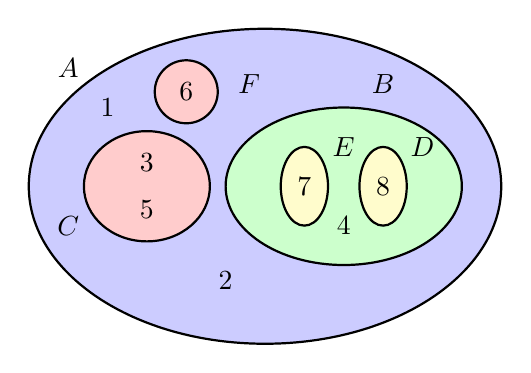
\begin{tikzpicture}[scale=1]
    % Definição dos conjuntos
    \draw[thick, fill=blue!20] (0,0) ellipse (3 and 2); % Conjunto maior (A)
    \draw[thick, fill=green!20] (1,0) ellipse (1.5 and 1); % Subconjunto de A (B)
    \draw[thick, fill=red!20] (-1.5,0) ellipse (0.8 and 0.7); % Subconjunto de A (C)
    \draw[thick, fill=red!20] (-1,1.2) ellipse (0.4 and 0.4); % Subconjunto de A (F)
    \draw[thick, fill=yellow!20] (0.5,0) ellipse (0.3 and 0.5); % Subconjunto de B (D)
    \draw[thick, fill=yellow!20] (1.5,0) ellipse (0.3 and 0.5); % Subconjunto de B (E)

    % Números dentro dos conjuntos
    \node at (-2, 1) {1}; % Elemento em A
    \node at (-0.5, -1.2) {2}; % Elemento em A
    \node at (-1.5, 0.3) {3}; % Elemento em B
    \node at (1.0, -0.5) {4}; % Elemento em B
    \node at (-1.5, -0.3) {5}; % Elemento em C
    \node at (-1, 1.2) {6}; % Elemento em F
    \node at (0.5, 0) {7}; % Elemento em D
    \node at (1.5, 0) {8}; % Elemento em E

    % Rótulos dos conjuntos
    \node at (-2.5, 1.5) {\( A \)}; % Rótulo para o conjunto A
    \node at (1.5, 1.3) {\( B \)}; % Rótulo para o conjunto B
    \node at (-2.5, -0.5) {\( C \)}; % Rótulo para o conjunto C
    \node at (2, 0.5) {\( D \)}; % Rótulo para o conjunto D
    \node at (1, 0.5) {\( E \)}; % Rótulo para o conjunto E
    \node at (-0.2, 1.3) {\( F \)}; % Rótulo para o conjunto F
\end{tikzpicture}
\caption{A figura ilustra uma coleção laminar $\{A, B, C, D, E, F\}$
de conjuntos, onde
$A := \{1,2,3,4,5,6,7,8\}$, $B := \{4, 7, 8\}$, $C := \{3, 5\}$,
$D := \{8\}$, $E := \{7\}$, $F := \{6\}$.
}
\end{figure}

Seja $(D, w \ge 0, r)$ um $r$-digrafo ponderado.
Para cada subconjunto $X \subseteq V$ e cada $F \subseteq A(D)$, seja 
\[
  \varrho_F(X) := |F \cap \delta^-(X)|,
\]
isto é, $\varrho_F(X)$ é o número de arcos de $F$ que \emph{entram} em $X$.
Para cada $k \in \mathbb{N}$, seja
\[
  [k) := \{\, i \in \mathbb{N} : i < k \,\}.
\]
Assim, por exemplo, $[4) = \{0,1,2,3\}$.
Uma sequência
\[
  \bigl( (R_i, \lambda_i) \bigr)_{i \in [k)},
\]
em que, para cada $i \in [k)$, o conjunto $R_i$ é um $r$-conjunto%
\footnote{Recorde que um $r$-conjunto é um subconjunto não vazio de $V$ que
  \emph{não} contém $r$.}
e $\lambda_i$ é um real não negativo, é dita \textbf{$w$-disjunta} se
\[
  \sum_{i \in [k)} \lambda_i \,[a \in \delta^-(R_i)] \;\le\; w(a)
\]
para cada $a \in A(D)$, em que $[\mathtt{P}]$ denota a função indicadora da
proposição $\mathtt{P}$, isto é, $[\mathtt{P}] = 1$ se $\mathtt{P}$ é verdadeira
e $[\mathtt{P}] = 0$ caso contrário. O número $\sum_{i \in [k)} \lambda_i$
é chamado de $\textbf{valor}$ da sequência $w$-disjunta $\bigl( (R_i, \lambda_i) \bigr)_{i \in [k)}$.


\begin{figure}[htb]
\centering
\begin{tikzpicture}[
    >=Stealth,
    vertex/.style={circle,draw,inner sep=1pt,font=\small},
    arc/.style={->,thick},
    rset/.style={draw=blue!60,thick},
    label/.style={font=\small},
    weight/.style={font=\small}
]

  %-------------------------------
  % Vértices e arco a
  %-------------------------------
  \node[vertex] (u) at (-2,0) {$u$};
  \node[vertex] (v) at ( 2.5,0) {$v$};

  \draw[arc] (u) -- node[weight,above,yshift=1pt,xshift=-1pt]
    {$a, 5$} (v);

  %-------------------------------
  % r-conjuntos laminares com v dentro
  % R1 ⊂ R2 ⊂ R3
  %-------------------------------
  % menor
  \draw[rset] (v) ellipse (0.8cm and 0.7cm);
  \node[label,blue!70,anchor=west]
    at ($(v)+(0.5,0.6)$) {$R_1, 2$};

  % intermediário
  \draw[rset] (v) ellipse (1.8cm and 1.2cm);
  \node[label,blue!70,anchor=west]
    at ($(v)+(1.7,0.0)$) {$R_2, 1$};

  % maior
  \draw[rset] (v) ellipse (2.8cm and 1.7cm);
  \node[label,blue!70,anchor=west]
    at ($(v)+(2.6,-0.6)$) {$R_3, 1$};

  %-------------------------------
  % Texto da desigualdade
  %-------------------------------

\end{tikzpicture}
\caption{Um arco $a$ de peso $5$ que entra nos $r$-conjuntos 
$R_1$, $R_2$ e $R_3$ com multiplidades $2$, $1$, e $1$, respectivamente.
}
\label{fig:w-disjunta-arco}
\end{figure}

Podemos pensar nos valores $\lambda_i$ como uma multiplicidade, no seguinte sentido.
Para cada $r$-conjunto $R_i$, o valor $\lambda_i$ representa a multiplicidade de $R_i$, isto é,
o “número de cópias” de $R_i$ que queremos incluir.
Além disso, fixado um arco $a$, o número total de vezes que $a$ é coberto pelos $\lambda_i$,
isto é, o valor
\[
  \sum_{i \in [k)} \lambda_i\,[a \in \delta^-(R_i)],
\]
não excede $w(a)$.



Suponha que $F$ é uma cobertura de $r$-conjuntos -- assim, para cada $r$-conjunto
$R$, vale $\varrho_F(R) \ge 1$ -- de $D$ e que
a sequência $\bigl( (R_i, \lambda_i) \bigr)_{i \in [k)}$ é $w$-disjunta.
Então
\begin{align*}
w(F) &= \sum_{a \in F} w(a) \\
     &\ge \sum_{a \in F} \sum_{i \in [k)} \lambda_i [a \in \delta^-(R_i)] \\
     &= \sum_{i \in [k)} \lambda_i \sum_{a \in F} [a \in \delta^-(R_i)] \\
     &= \sum_{i \in [k)} \lambda_i \,\varrho_F(R_i) \\
     &\ge \sum_{i \in [k)} \lambda_i.
\end{align*}
Na última desigualdade usamos que $F$ é uma cobertura de $r$-conjuntos,
de modo que, para cada $i \in [k)$, vale $\varrho_F(R_i) \ge 1$.

Note que $w(F) = \sum_{i \in [k)} \lambda_i$ se, e somente se,
há igualdade em todas as desigualdades na cadeia acima. Logo,
\[
  w(F) = \sum_{i \in [k)} \lambda_i
\]
se, e somente se, as seguintes \textbf{condições de otimalidade} valem:
\begin{subequations}\label{eq:condicoes-otimalidade}
\begin{align}
\forall a \in F:\quad 
  & w(a) = \sum_{i \in [k)} \lambda_i\,[a \in \delta^-(R_i)], 
    \label{eq:condicao-arcos} \\
\forall i \in [k):\quad 
  & \varrho_F(R_i) = 1. 
    \label{eq:condicao-conjuntos}
\end{align}
\end{subequations}


Assim, se $F$ é uma $r$-arborescência geradora e
$\bigl((R_i, \lambda_i)\bigr)_{i \in [k)}$
é uma sequência $w$-disjunta que satisfaz as condições de otimalidade~\eqref{eq:condicoes-otimalidade}, então
$F$ é uma $r$-arborescência de peso mínimo e 
$\bigl((R_i, \lambda_i)\bigr)_{i \in [k)}$ é uma sequência $w$~-~disjunta de valor máximo.%
\footnote{Isto é, $\sum_{i \in [k)} \lambda_i$ é máximo entre todas
as sequências $w$-disjuntas.}


\section{Fase 1 do algoritmo de Frank}

Antes de iniciarmos a descrição da fase 1, vale destacar que,
embora ela seja referida como a fase 1 do algoritmo de Frank,
ela é, na verdade, essencialmente devida a Fulkerson~\cite{fulkerson}.

 
É conveniente introduzir a seguinte definição para simplificar a notação.
Seja $U$ um conjunto e seja $X \subseteq U$.
Definimos $\mathbf{1}^U_X : U \to \{0,1\}$ pondo
\[
  \mathbf{1}^U_X(u) :=
  \begin{cases}
    1, & \text{se } u \in X,\\
    0, & \text{caso contrário},
  \end{cases}
\]
para cada $u \in U$. 
Quando o contexto permitir, escrevemos $\mathbf{1}_X$ no lugar de $\mathbf{1}^U_X$.
Além disso, se $\lambda \in \mathbb{R}$ e
$f : U \to \mathbb{R}$, então $\lambda f : U \to \mathbb{R}$ é definida pondo
\[
  (\lambda f)(u) := \lambda\, f(u)
\]
para cada $u \in U$. Finalmente, como de costume, se $g : U \to \mathbb{R}$,
então $f - g : U \to \mathbb{R}$ é definida pondo
\[
  (f - g)(u) := f(u) - g(u)
\]
para cada $u \in U$.


Voltemos à descrição da primeira fase.
A apresentação dessa fase, bem como dos demais algoritmos
deste capítulo, segue de perto a exposição informal, porém rigorosa,
de~\cite{feofiloff}.



Seja $(D, w \ge 0, r)$ um $r$-digrafo ponderado.
A primeira fase do algoritmo constrói uma sequência
\[
  \bigl((f_i, R_i, \lambda_i)\bigr)_{i \in [k)}
\]
que satisfaz as seguintes condições:
\begin{subequations}\label{eq:fase1-condicoes}
\begin{gather}
\{f_i : i \in [k)\} 
  \text{ é uma cobertura de $r$-conjuntos de $D$}, 
  \label{eq:fase1-cobertura} \\[4pt]
\bigl((R_i, \lambda_i)\bigr)_{i \in [k)} 
  \text{ é uma sequência $w$-disjunta}, 
  \label{eq:fase1-w-disjunta} \\[4pt]
\forall j \in [k):\quad
  \sum_{i \in [k)} \lambda_i\,[f_j \in \delta^-(R_i)] 
  = w(f_j).
  \label{eq:fase1-arcos}
\end{gather}
\end{subequations}
Note que~\eqref{eq:fase1-arcos} é a condição~\eqref{eq:condicao-arcos}.

Cada iteração da primeira fase começa com uma função $c: A \to \mathbb{R}_+$ e uma  
sequência $\bigl((f_i, R_i, \lambda_i)\bigr)_{i \in [k)}$ tais que
\begin{subequations}\label{eq:iter:fase1-condicoes}
\begin{gather}
c = w - \sum_{i \in [k)} \lambda_i \mathbf{1}_{\delta^-(R_i)}
\label{eq:iter:c e w} \\[4pt]
\forall i \in [k):\quad
  f_i \text{ entra em } R_i,
  \label{eq:iter:fase1-cobertura} \\[4pt]
\forall i \in [k),\ \forall j \in [i):\quad
  f_j \text{ \emph{não} entra em } R_i,
  \label{eq:iter:fase1-prioridade} \\[4pt]
\forall i \in [k),\ \forall \varnothing \subset R \subset R_i,\ \exists h \in [i): 
\quad f_h \text{ entra em } R,
\label{eq:iter:fase1-subcover} \\[4pt]
\bigl((R_i, \lambda_i)\bigr)_{i \in [k)} 
  \text{ é uma sequência $w$-disjunta},
  \label{eq:iter:fase1-w-disjunta} \\[4pt]
\{R_i : i \in [k)\}
  \text{ é uma coleção laminar de $r$-conjuntos},
  \label{eq:iter:fase1-laminar} \\[4pt]
\forall i \in [k):\quad c(f_i) = 0
  \label{eq:iter:fase1-arcos}
\end{gather}
\end{subequations}
Note que a condição~\eqref{eq:iter:fase1-arcos} é equivalente a
\[ \forall i \in [k):\quad 
  \sum_{j \in [k)} \lambda_j\,[f_i \in \delta^-(R_j)] 
  = w(f_i).
\]
A primeira iteração começa com $c = w$ e com a sequência vazia. 
Cada iteração consiste no seguinte.
Suponha que $\sigma := \bigl((f_i, R_i, \lambda_i)\bigr)_{i \in [k)}$
satisfaz~\eqref{eq:iter:fase1-condicoes}.
Se $F := \{f_i : i \in [k)\}$ é uma cobertura de $r$-conjuntos de $D$, então
o algoritmo pára e devolve $\sigma$. Suponha que esse não seja o caso.
O algoritmo então seleciona um $r$-conjunto \emph{minimal} $R_k$ que não é coberto por $F$.
Como $D$ possui ao menos uma $r$-arborescência, então existe ao menos um arco que
entra em $R_k$.
A próxima iteração começa com
$\sigma \cdot (f_k, R_k, \lambda_k)$ no lugar de $\sigma$
e $c - \lambda_k \mathbf{1}_{\delta^-(R_k)}$ no lugar de $c$, em que
\begin{itemize}
\item $\lambda_k := 
  \min \Bigl\{\, 
    c(a) a \in \delta^-(R_k)
  \Bigr\}$, e
\item $f_k$ é um arco em $\delta^-(R_k)$ tal que $c(f_k) = \lambda_k$.
\end{itemize}


Precisamos verificar que $\sigma \cdot (f_k, R_k, \lambda_k)$
satisfaz~\eqref{eq:iter:fase1-condicoes}.
A única propriedade em~\eqref{eq:iter:fase1-condicoes} que não segue
diretamente das escolhas de $f_k$, $R_k$ e $\lambda_k$
é a laminaridade da coleção $\{R_i : i \in [k+1)\}$.
Suponha que esse não seja o caso.
Então existe $i \in [k)$ tal que 
\[
  R_i \cap R_k \neq \varnothing,\quad
  R_i \setminus R_k \neq \varnothing,\quad
  R_k \setminus R_i \neq \varnothing.
\]
Em virtude de~\eqref{eq:iter:fase1-subcover}, existe $h \in [i)$ tal que
$f_h =: uv$ entra em $R_i \cap R_k$. Assim, $u \notin R_i \cap R_k$ e
$v \in R_i \cap R_k$.
Ora, $u \notin R_i \cap R_k$ implica que $u \in V \setminus R_i$ ou $u \in V \setminus R_k$.
Mas $u \in V \setminus R_i$ implica que $uv$ entra em $R_i$, o que contraria
\eqref{eq:iter:fase1-prioridade}. Por outro lado, $u \in V \setminus R_k$ implica
que $uv$ entra em $R_k$, o que novamente é uma contradição, pois $F$ não entra em $R_k$.
Logo, a coleção $\{R_i : i \in [k+1)\}$ é laminar.


Para completar a descrição da primeira fase, basta mostrar como
encontrar um $r$-conjunto minimal que não é coberto por $F$.
Para isso, considere o digrafo $D_0 := (V, F)$.
Como $F$ não é uma cobertura de $r$-conjuntos, $D_0$ não contém
uma $r$-arborescência. Logo, pela
Proposição~\ref{prop:car:arb}, existe um $r$-conjunto $X \subseteq V$
tal que nenhum arco de $F$ entra em $X$. Logo, existe pelo menos
uma fonte, digamos $S$, em $\mathcal{C}(D_0)$. Proposição~\ref{prop:minimal:ent}, 
$S$ é um $r$-conjunto minimal não coberto por $F$.

\begin{proposicao}
\label{prop:minimal:ent}
Seja $H$ um digrafo e seja $r$ um vértice de $H$.
Para toda fonte $S$ de $\mathcal{C}(H)$, se $r \notin S$, então 
$S$ é um $r$-conjunto minimal não coberto por $A(H)$.  
\end{proposicao}

\begin{proof}[Prova.]
Suponha que $S$ seja uma fonte de $\mathcal{C}(H)$ que satisfaz $r \notin S$. 
Como $S$ é uma fonte de $\mathcal{C}(H)$, nenhum arco de $H$ entra em $S$.
Além disso, $r \notin S$, donde $S$ é um $r$-conjunto não coberto por $A(H)$.
Resta mostrar que $S$ é minimal.

Ora, $S$ é uma componente fortemente conexa de $H$,
de modo que $H[S]$ é fortemente conexo.
Seja agora $\emptyset \neq R \subset S$ um subconjunto próprio e não vazio de $S$.
Como $H[S]$ é fortemente conexo, existe ao menos um arco de $H[S]$ que entra em $R$.
Como $A(H[S]) \subseteq A(H)$, esse arco pertence a $A(H)$ e entra em $R$.
Logo, $A(H)$ entra em todo subconjunto próprio e não vazio de $S$.

Portanto, $S$ não é coberto por $A(H)$, mas todo subconjunto próprio não vazio de $S$
é coberto por $A(H)$, isto é, $S$ é um $r$-conjunto minimal não coberto por $A(H)$.
\end{proof}

\begin{figure}[htb]
\centering
\begin{tikzpicture}[
    >=Stealth,
    vertex/.style={circle,draw,inner sep=1pt,font=\small},
    blackarc/.style={->,thin,black},                % arcos pretos de D
    greenarc/.style={->,very thick,green!60!black}, % arcos verdes (subdigrafo)
    sccbox/.style={draw=blue!60,rounded corners,inner sep=4pt,dashed},
    info/.style={draw=none,font=\small}
]

  % -----------------------------
  % Vértice raiz
  % -----------------------------
  \node[vertex] (r) at (0,3.0) {$r$};

  % -----------------------------
  % Componente forte C1 (esquerda): a,b,g
  % -----------------------------
  \node[vertex] (a) at (-3,1.2) {$a$};
  \node[vertex] (b) at (-2,0.2) {$b$};
  \node[vertex] (g) at (-3,-0.8) {$g$};

  % -----------------------------
  % Componente forte C2 (direita): c,d,h
  % -----------------------------
  \node[vertex] (c) at ( 3,1.2) {$c$};
  \node[vertex] (d) at ( 2,0.2) {$d$};
  \node[vertex] (h) at ( 3,-0.8) {$h$};

  % -----------------------------
  % Componente forte C3 (baixo): e,f
  % -----------------------------
  \node[vertex] (e) at (-0.9,-2.0) {$e$};
  \node[vertex] (f) at ( 0.9,-2.0) {$f$};

  % -----------------------------
  % Arcos pretos de D (genéricos)
  % -----------------------------
  \draw[blackarc] (r) -- (a);
  \draw[blackarc] (r) -- (c);
  \draw[blackarc] (r) -- (e);

  %\draw[blackarc] (g) .. controls (-1.5,2.0) .. (r);
  %\draw[blackarc] (h) .. controls ( 1.5,2.0) .. (r);
  \draw[blackarc] (e) .. controls (0.0,-0.2) .. (d);

  % -----------------------------
  % Arcos verdes (subdigrafo D[B])
  % -----------------------------
  % C1: ciclo forte a -> b -> g -> a (fonte na condensação)
  \draw[greenarc] (a) -- (b);
  \draw[greenarc] (b) -- (g);
  \draw[greenarc] (g) -- (a);

  % C2: ciclo forte c -> d -> h -> c (outra fonte)
  \draw[greenarc] (c) -- (d);
  \draw[greenarc] (d) -- (h);
  \draw[greenarc] (h) -- (c);

  % C3: e <-> f, agora com curvaturas opostas
  \draw[greenarc,bend left=20] (e) to (f);
  \draw[greenarc,bend left=20] (f) to (e);

  % Arcos verdes entre componentes: C1 -> C3, C2 -> C3
  \draw[greenarc] (b) .. controls (-1.8,-1.0) .. (e);
  \draw[greenarc] (d) .. controls ( 1.8,-1.0) .. (f);

  % -----------------------------
  % Caixas destacando C1, C2, C3
  % -----------------------------
  \node[sccbox,fit=(a) (b) (g)] (C1box) {};
  \node[sccbox,fit=(c) (d) (h)] (C2box) {};
  \node[sccbox,fit=(e) (f)]     (C3box) {};

  \node[info,blue!60,above left=0pt of C1box.north west] {$C_1$};
  \node[info,blue!60,above right=0pt of C2box.north east] {$C_2$};
  \node[info,blue!60,below=1pt of C3box.south] {$C_3$};

\end{tikzpicture}
\caption{Digrafo $D$ com raiz $r$: arcos pretos em $A(D)\setminus F$ e
arcos verdes em $F$. 
As caixas tracejadas destacam os componentes fortemente
conexos de $D[F]$; $C_1$ e $C_2$ são fontes na condensação.}
\label{fig:fontes-condensacao-verde}
\end{figure}

Para sumarizar o processo algoritmo recém descrito,
eis um pseudo-código da fase 1 do algoritmo de Frank.

\begin{tcolorbox}[
		enhanced, breakable,
		colframe=blue!60!black, colback=blue!2,
		colbacktitle=blue!15, coltitle=black,
		title={Fase 1 do algoritmo de Frank (algoritmo de Fulkerson)},
		boxed title style={sharp corners, boxrule=0.6pt},
		sharp corners, boxrule=0.6pt
	]
	\emph{Recebe um $r$-digrafo ponderado $(D, w, r)$ e devolve uma sequência
	$\sigma$ que satisfaz~\eqref{eq:fase1-condicoes}.}
	\tcblower
	\begin{lstlisting}[language=Python, mathescape=true]
def phase1($D$, $w$, $r$):
    $c, \sigma := w, \epsilon$
    loop:
        $(f_i, R_i, \lambda_i)_{i \in [k)} := \sigma$
        $F := \{f_i \mid i \in [k)\}$
        $D_0 := (V, F)$
        if $\mathcal{C}(D_0)$ não possui fontes: return $\sigma$
        seja $R_k$ uma fonte em $\mathcal{C}(D_0)$
	    $\lambda_k := \min \{ c(a) : a \in \delta^-(R_k) \}$
	    seja $f_k \in \delta^-(R_k)$ tal que $c(f_k) = \lambda_k$
	    $\sigma := \sigma \cdot (f_k, R_k, \lambda_k)$
	    $c := c - \lambda_k \mathbf{1}_{\delta^-(R_k)}$
\end{lstlisting}
\end{tcolorbox}

\subsection*{Complexidade}

A cada iteração, o algoritmo determina um componente fonte de $\mathcal{C}(D_0)$,
o que pode ser realizado em tempo $O(|A|)$, usando, por exemplo, o algortimo de Kosaraju~\cite{clrs}. O conjunto obtido da sequência de $r$-conjunto devolvida pelo algoritmo é laminar (e a sequência não possui repetições). Logo, seu tamanho é limitado por $2|V| - 1$.
Consequentemente, é possível implementar a fase 1 em tempo $O(|V||A|)$.


\section{Implementação da fase 1}

A função \texttt{phase1} recebe \texttt{D: DiGraph}, ponderado pelo atributo
\texttt{"w"} associado a cada arco, e \texttt{r: int}, que é um vértice de
\texttt{D}. Além disso, \texttt{D} deve possuir uma \texttt{r}-arborescência.
A função devolve uma lista \texttt{sigma} de triplas que corresponde
à sequência $\lambda$ satisfazendo~\eqref{eq:fase1-condicoes}.

Na linha 3, é definido \texttt{D\_zero}, que, durante a execução da função,
armazena os arcos da lista \texttt{sigma} — mais precisamente, o primeiro
componente de cada tripla em \texttt{sigma}. Assim, em cada iteração, temos
\(\texttt{D\_zero} = (V, F)\), onde \(F = \{f_i\}\) é a família de arcos já
selecionados.

A função usa \texttt{condensation}, da biblioteca \texttt{NetworkX}, que recebe
um \texttt{DiGraph} e devolve um \texttt{DiGraph} que é a sua condensação. Assim,
após a execução da linha 5, \texttt{C} é a condensação de \texttt{D\_zero}. Na
linha 6, as fontes de \texttt{C}, isto é, os vértices nos quais nenhum arco
entra, são coletadas na lista \texttt{sources}. 

Pela hipótese de que \((D,w,r)\) admite uma $r$-arborescência, sabemos que toda
fonte de \(\mathcal{C}(D_0)\) que não contém \(r\) corresponde a um
$r$-conjunto minimal não coberto. Logo, quando \texttt{sources} contém apenas
uma fonte, todos os $r$-conjuntos já estão cobertos e a função termina.

Caso contrário, para cada fonte de \texttt{C}, os vértices do componente forte
correspondente em \texttt{D\_zero} são coletados em \texttt{X} (linha 9); um tal
\texttt{X} é de interesse desde que \texttt{r} não pertença a \texttt{X}. Nesse
caso, os arcos de \texttt{D\_copy} que entram em \texttt{X} são armazenados em
\texttt{arcs} (linha 12). O peso de um arco de custo mínimo em \texttt{arcs} é
determinado na linha 15 e armazenado em \texttt{min\_weight}.

A função \texttt{update\_weights} decrementa de \texttt{min\_weight} o peso de
cada arco em \texttt{arcs} e devolve um arco de menor peso em \texttt{arcs}, que
é armazenado em \texttt{a} (linha 16). O arco \texttt{a} é adicionado ao
digrafo \texttt{D\_zero} (linha 17). Finalmente, na linha 18, a tripla
\texttt{(a, X, min\_weight)} é adicionada à lista \texttt{sigma}.


\begin{tcolorbox}[
		enhanced, breakable,
		colframe=blue!60!black, colback=blue!2,
		colbacktitle=blue!15, coltitle=black,
		title={Fase 1 do algoritmo de Frank},
		boxed title style={sharp corners, boxrule=0.6pt},
		sharp corners, boxrule=0.6pt
	]
	\emph{Entrada:} \texttt{D: DiGraph}, \texttt{r: int}
	
	\emph{Pré-condição:} \texttt{D} é ponderado, \texttt{r} é um vértice de \texttt{D},
	e \texttt{D} possui uma \texttt{r}-arborescência.
	
	\emph{Saída:} uma lista \texttt{sigma} que corresponde à uma sequência 
	que satisfaz~\ref{eq:fase1-condicoes}.
	\tcblower
	\begin{lstlisting}[language=Python, basicstyle=\ttfamily\fontsize{8}{9}\selectfont]
def phase1(D: nx.DiGraph, r: int):
    D_copy = D.copy()
    sigma = []
    D_zero = nx.DiGraph(); D_zero.add_nodes_from(D_copy.nodes())
    while True:
        C = nx.condensation(D_zero)
        sources = [x for x in C.nodes() if C.in_degree(x) == 0]
        if len(sources) == 1: break
        for s in sources:
            X = C.nodes[s]["members"]
            if r in X:
                continue
            arcs = [(u, v, data) 
                    for u, v, data in D_copy.edges(data=True) 
                    if u not in X and v in X]
            min_weight = min(data["w"] for _, _, data in arcs)
            a = update_weights(D_copy, arcs, min_weight)
            D_zero.add_edge(a[0], a[1])
            sigma.append((a, X, min_weight)) 
    return sigma
\end{lstlisting}
\end{tcolorbox}

A função \texttt{update\_weights} é muito simples e segue abaixo.

\begin{tcolorbox}[
		enhanced, breakable,
		colframe=blue!60!black, colback=blue!2,
		colbacktitle=blue!15, coltitle=black,
		title={Fase 1 do algoritmo de Frank},
		boxed title style={sharp corners, boxrule=0.6pt},
		sharp corners, boxrule=0.6pt
	]
	\emph{Entrada:} \texttt{D: DiGraph}, \texttt{arcs: list[tuple[int, int, dict]]},
		            \texttt{min\_weight: float}.
	
	\emph{Pré-condição:} \texttt{D} é ponderado, \texttt{arcs} é uma lista de arcos,
	\texttt{min\_weight} é o peso de um arco de menor peso em \texttt{arcs}.
	
	\emph{Pós-condição:} Decrementa de \texttt{min\_weight} o peso de cada arco em \texttt{arcs},
	modificando esse atributo em \texttt{D}. 

	\tcblower
	\begin{lstlisting}[language=Python, basicstyle=\ttfamily\fontsize{8}{9}\selectfont]
def update_weights(D: nx.DiGraph, 
                   arcs: list[tuple[int, int, dict]],
                   min_weight: float):
    for u, v, _ in arcs:
        D[u][v]["w"] -= min_weight
        if D[u][v]["w"] == 0:
            a = (u, v)
    return a
\end{lstlisting}
\end{tcolorbox}


\section{Fase 2 do Algoritmo de Frank}

A fase 2 do algoritmo de Frank recebe um $r$-digrafo ponderado $(D, w \ge 0, r)$
e uma sequência $(f_i)_{i \in [k)}$ extraída da sequência
$\bigl((f_i, R_i, \lambda_i)\bigr)_{i \in [k)}$, obtida na fase 1 do algoritmo
de Frank, a qual satisfaz~\eqref{eq:fase1-condicoes}.
A fase 2 devolve um subconjunto $J \subseteq \{f_i : i \in [k)\}$ que é uma
$r$-arborescência geradora de $D$, satisfazendo~\eqref{eq:condicao-arcos},
ou seja,%
\footnote{Se preferir em palavras, isto quer dizer que, em cada $r$-conjunto $R_i$,
entra exatamente um arco de $J$.}
\[
  \forall i \in [k):\quad \varrho_J(R_i) = 1.
\]
A combinação da sequência $\bigl((R_i, \lambda_i)\bigr)_{i \in [k)}$ com esse
conjunto $J$ prova que $J$ é uma $r$-arborescência geradora de peso mínimo
de $(D, w)$.


Cada iteração da fase 2 começa com um conjunto $J$ de arcos tal que $J$ é uma
$r$-arborescência.%
\footnote{Assuma, por simplicidade, que quando $J = \varnothing$ o digrafo $J$
é uma $r$-arborescência.}
A primeira iteração começa com $J := \varnothing$.
Cada iteração consiste no seguinte.
Se $J$ é uma $r$-arborescência geradora, então o algoritmo pára e devolve $J$.
Suponha que esse não seja o caso.
O algoritmo então considera a sequência
\[
  (f_i)_{i \in [k)}
\]
e seleciona o menor $i \in [k)$ tal que $f_i$ é um arco que sai de $V(J)$.
Note que tal arco deve existir, pois $\{f_i : i \in [k)\}$ é uma cobertura
de $r$-conjuntos.
A próxima iteração começa com $J \cup \{f_i\}$ no lugar de $J$.


Afirmamos que no início de cada iteração, o conjunto $J$ satisfaz
\[ \forall i \in [k): \varrho_J(R_i) \le 1. \]
Isso é óbvio no início da primeira iteração.
Considere uma iteração arbitrária e suponha que $J$ não é uma $r$-arborescência.
Vamos mostrar que $J \cup \{f_i\}$ satisfaz
\[ \forall i \in [k): \varrho_{J \cup \{f_i\}}(R_i) \le 1. \]
Por construção, dentre os arcos de $(f_i)_{i \in [k)}$ que saem de $V(J)$,
o arco $f_i$ é o de menor índice. Além disso, $f_i$ entra em $R_i$.
Suponha, por um momento, que algum arco de $J$ entre em $R_i$; 
então $V(J) \cap R_i \neq \varnothing$,
donde $R_i \setminus V(J) \subset R_i$.
Além disso, como $f_i$ sai de $V(J)$ e entra em $R_i$, concluímos que
$R_i \setminus V(J) \neq \varnothing$. Logo, $\varnothing \subset R_i \setminus V(J) \subset R_i$.

Sabemos que, para cada $\varnothing \subset R \subset R_i$, existe um arco de 
$F := \{ f_j : j \in [k)\}$
que entra em $R$ e cujo índice é menor que $i$. Em particular, tomando
$R := R_i \setminus V(J)$, existe $f_k =: uv \in F$ tal que $f_k$ entra em
$R_i \setminus V(J)$ e, portanto, $k < i$ e $v \in R_i \setminus V(J)$.
Como $f_k$ não entra em $R_i$ e a ponta final $v$ pertence a $R_i$, segue que
$u \in R_i$.

Ora, $
  R_i = (R_i \cap V(J)) \cup (R_i \setminus V(J)),
$
e, como $u \in R_i$ e $u \notin R_i \setminus V(J)$, obtemos $u \in V(J)$.
Logo, $f_k$ é um arco de $F$ que sai de $V(J)$, o que contraria a escolha de $i$,
pois $k < i$.
Essa contradição mostra que $J \cup \{f_i\}$ satisfaz
\[ \forall i \in [k): \varrho_{J \cup \{f_i\}}(R_i) \le 1, \]
como queríamos.


O pseudo-código do algoritmo da fase 2, em uma versão ingênua,
é muito simples.

\begin{tcolorbox}[
		enhanced, breakable,
		colframe=blue!60!black, colback=blue!2,
		colbacktitle=blue!15, coltitle=black,
		title={Fase 2: Construção da $r$-arborescência geradora},
		boxed title style={sharp corners, boxrule=0.6pt},
		sharp corners, boxrule=0.6pt
	]
	\emph{Recebe um digrafo $D$, um vértice $r$ de $D$ e
	uma sequência  $(f_i)_{i \in [k)}$ de arcos 
	tal que $\{f_i : i \in [k)\}$ é uma cobertura dos $r$-conjuntos de $D$, 
	e devolve um subdigrafo que é uma $r$-arborescência geradora de $D$.}
	\tcblower
	\begin{lstlisting}[language=Python, mathescape=true]
def phase2($D$, $r$, $(f_i)_{i \in [k)}$):
    $U, J := \{r\}, \varnothing$
    for $t := 1$ to $|V(D)|-1$:
        for $i \in [k)$:
            $(u_i, v_i) := f_i$
            if $u_i \in U$ e $v_i \notin U$:
                $U, J := U \cup \{v_i\}, J \cup \{f_i\}$
                break
    return $(U, J)$
\end{lstlisting}
\end{tcolorbox}

\subsection*{Complexidade}

Observe que o algoritmo realiza $O(|V(D)|)$ iterações e que
cada iteração pode ser implementada de modo a consumir tempo
em $O(|F|)$. Logo, o consumo de tempo está em $O(|V||F|)$.

\section{Implementação da fase 2}

A implemantação da fase 2 é muito simples e segue bem de perto 
a versão do pseudo-código.

\begin{tcolorbox}[
		enhanced, breakable,
		colframe=blue!60!black, colback=blue!2,
		colbacktitle=blue!15, coltitle=black,
		title={Fase 2: Construção da arborescência},
		boxed title style={sharp corners, boxrule=0.6pt},
		sharp corners, boxrule=0.6pt
	]
	\emph{Entrada:} \texttt{D: nx.DiGraph}, \texttt{r: int}, 
	\texttt{F: list[tuple[int, int]]} 
	
	\emph{Pré-condição:} \texttt{F} é uma cobertura de \texttt{r}-conjuntos de \texttt{D}.
	
    \emph{Saída:} Um \texttt{DiGraph} que é uma \texttt{r}-arborescência geradora de \texttt{D} cujos arcos estão contidos em \texttt{F}. 	

\tcblower
\begin{lstlisting}[language=Python]
def phase2(D: nx.DiGraph, r: int, F: list[tuple[int, int]]):
    Arb = nx.DiGraph()
    Arb.add_node(r)
    n = len(D.nodes())
    for _ in range(n - 1):
        for u, v in F:
            if u in Arb.nodes() and v not in Arb.nodes():
                edge_data = D.get_edge_data(u, v)
                Arb.add_edge(u, v, **edge_data)
                break
    return Arb
\end{lstlisting}
\end{tcolorbox}

\section{Versão alternativa da fase 2}

Vamos agora exibir uma versão alternativa e mais eficiente da fase 2,
como sugerido em~\cite{pslr}, que fornece um algoritmo que pode ser 
implementado em tempo $O(|A| + |V|\log |V|)$. No contexto
do nosso problema isso se reduz a $O(|V|\lg|V|)$.
A ideia é simples e nada mais é do que uma variante do algoritmo de
Dijkstra~\cite{clrs}.

A versão alternativa recebe um $r$-digrafo ponderado $(D, w \ge 0, r)$
e uma sequência $(f_i)_{i \in [k)}$ extraída da sequência
$\bigl((f_i, R_i, \lambda_i)\bigr)_{i \in [k)}$, obtida na fase 1 do algoritmo
de Frank, a qual satisfaz~\eqref{eq:fase1-condicoes}.
Ela devolve um subconjunto $J \subseteq \{f_i : i \in [k)\}$ que é uma
$r$-arborescência geradora de $D$ e satisfaz~\eqref{eq:condicao-arcos}.

Forme o subdigrafo gerador
\[
  H := \bigl(V,\{f_i : i \in [k)\}\bigr)
\]
de $D$ e a função \emph{prioridade}
\[
  p : \{f_i : i \in [k)\} \to \mathbb{N}
  \quad\text{tal que}\quad
  p(f_i) := i \text{ para cada } i \in [k).
\]

Cada iteração do algoritmo começa com um subconjunto $J$ de arcos de $H$
e com um subconjunto $Q$ também de arcos de $H$.
A primeira iteração começa com
\[
  J := \varnothing
  \quad\text{e}\quad
  Q := \delta^+_H(r).
\]
Cada iteração consiste no seguinte.

\begin{itemize}
\item Se $Q = \varnothing$, então o algoritmo pára e devolve $J$.

\item Caso contrário, o algoritmo seleciona um arco $(u,v) \in Q$ tal que
      $p(u,v)$ é mínimo.

      \begin{itemize}
      \item Se $v \in V(J)$, então o algoritmo inicia uma nova iteração com
            $J$ e $Q \setminus \{(u,v)\}$ nos papéis de $J$ e $Q$,
            respectivamente.

      \item Se $v \notin V(J)$, então o algoritmo inicia uma nova iteração com
            \[
              J' := J \cup \{(u,v)\}
              \quad\text{e}\quad
              Q' := \bigl(Q \setminus \{(u,v)\}\bigr) \cup \delta^+_H(v)
            \]
            nos papéis de $J$ e $Q$, respectivamente.
      \end{itemize}
\end{itemize}

A implementação dessa versão segue abaixo.

\begin{tcolorbox}[
		enhanced, breakable,
		colframe=blue!60!black, colback=blue!2,
		colbacktitle=blue!15, coltitle=black,
		title={Versão alternativa da fase 2},
		boxed title style={sharp corners, boxrule=0.6pt},
		sharp corners, boxrule=0.6pt
	]
	\emph{Entrada:} \texttt{D: nx.DiGraph}, \texttt{r: int}, 
	\texttt{F: list[tuple[int, int]]} 
	
	\emph{Pré-condição:} \texttt{F} é uma cobertura de \texttt{r}-conjuntos de \texttt{D}.
	
    \emph{Saída:} Um \texttt{DiGraph} que é uma \texttt{r}-arborescência geradora de \texttt{D}
	\tcblower
	\begin{lstlisting}[language=Python]
def phase2_v2(D, r, F):
    Arb = nx.DiGraph()
    for i, (u, v) in enumerate(F):
        Arb.add_edge(u, v, w=i)
    V = {r}
    q = []
    for u, v, data in Arb.out_edges(r, data=True):
        heapq.heappush(q, (data["w"], u, v))
    J = nx.DiGraph()
    while q:
        _, u, v = heapq.heappop(q)
        if v in V:
            continue
        J.add_edge(u, v, w=D[u][v]["w"])
        V.add(v)
        for x, y, data in Arb.out_edges(v, data=True):
            heapq.heappush(q, (data["w"], x, y))
    return J
\end{lstlisting}
\end{tcolorbox}


\section{O algoritmo de Frank}

O algoritmo de Frank é obtido compondo-se as duas fases.
Há duas versões à disposição. Para obter a segunda, 
basta trocar a chamada da função \texttt{phase2\_v2} pela chamada
da função \texttt{phase2}. 

\begin{tcolorbox}[
		enhanced, breakable,
		colframe=blue!60!black, colback=blue!2,
		colbacktitle=blue!15, coltitle=black,
		title={Fase 2: Construção da $r$-arborescência geradora},
		boxed title style={sharp corners, boxrule=0.6pt},
		sharp corners, boxrule=0.6pt
	]
	\emph{Recebe um $r$-digrafo ponderado $(D, w, r)$, e
	devolve um par $\bigl(J, (R_i, \lambda_i)_{i \in [k)}\bigr)$
	satisfazendo as condições de otimalidade~\eqref{eq:condicoes-otimalidade}.}
	\tcblower
	\begin{lstlisting}[language=Python, mathescape=true]
def frankv1($D$, $w$, $r$):
    $(f_i, R_i, \lambda_i)_{i \in [k)} :=$ phase1($D$, $w$, $r$)
    $J :=$ phase2_v2($D$, $r$, $\{f_i : i \in [k)\}$)
    return $\bigl(J, (R_i, \lambda_i)_{i \in [k)}\bigr)$
\end{lstlisting}
\end{tcolorbox}

\section*{Complexidade}

O algoritmo \texttt{phase1} tem consumo de tempo em $O(|V||A|)$.
A sequência devolvida tem comprimento $k \le 2|V| - 1$.
Assim, o consumo de tempo de \texttt{phase2\_v2} está em $O(|V|\lg|V|)$.
Logo, o consumo de tempo de \texttt{frankv1} está em $O(|V|(\lg|V| + |A|))$.

